\section{dg::Set$<$ TYPE $>$ Class Template Reference}
\label{classdg_1_1Set}\index{dg::Set@{dg::Set}}
{\tt \#include $<$Set.h$>$}

Collaboration diagram for dg::Set$<$ TYPE $>$:\begin{figure}[H]
\begin{center}
\leavevmode
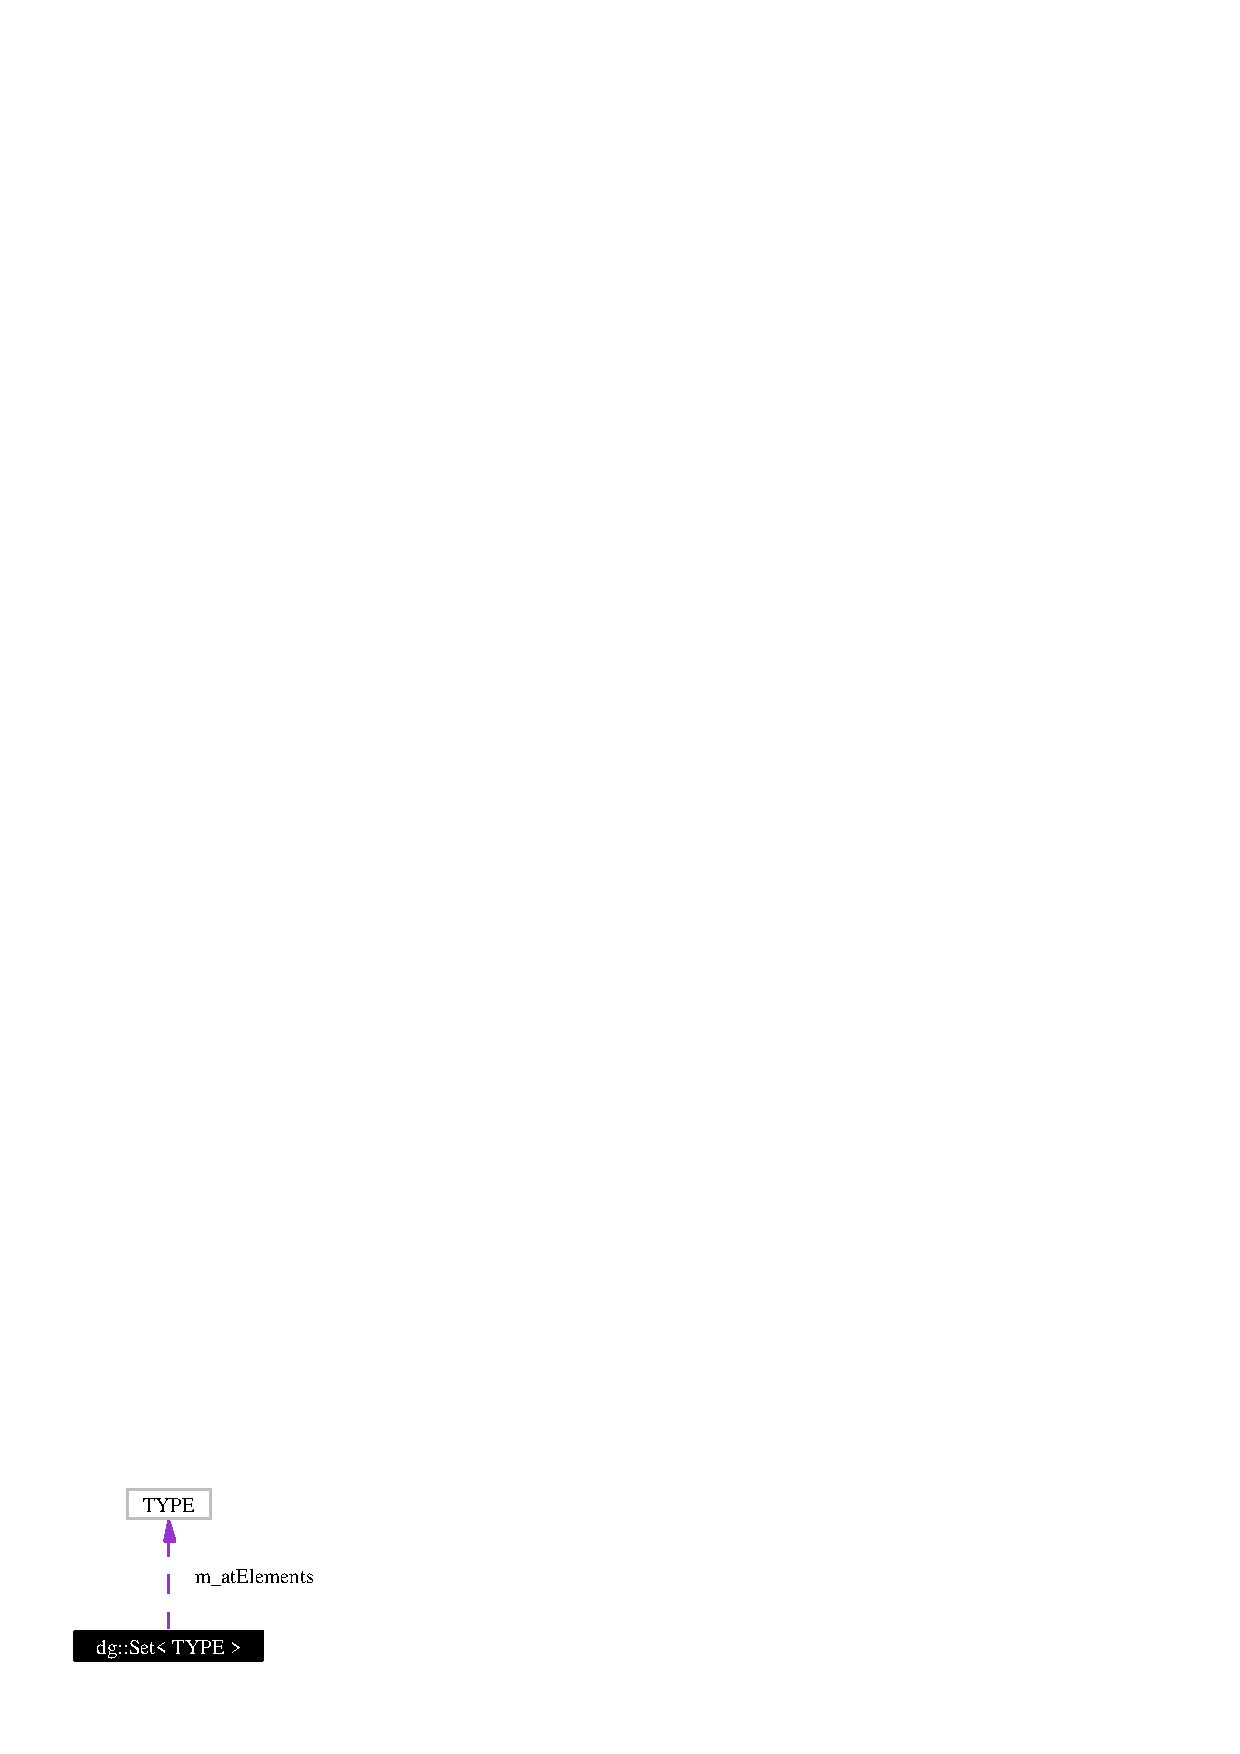
\includegraphics[width=81pt]{classdg_1_1Set__coll__graph}
\end{center}
\end{figure}
\subsubsection*{template$<$class TYPE$>$ class dg::Set$<$ TYPE $>$}

\subsection*{Public Methods}
\begin{CompactItemize}
\item 
{\bf Set} ({\bf UInt} i\-Capacity=1, {\bf UInt} i\-Resize=10)
\item 
{\bf Set} (const Set \&rk\-Set)
\item 
{\bf $\sim$Set} ()
\item 
Set \& {\bf operator=} (const Set \&rk\-Set)
\item 
{\bf UInt} {\bf capacity} () const
\item 
{\bf UInt} {\bf resize} () const
\item 
{\bf UInt} {\bf size} () const
\item 
const TYPE $\ast$ {\bf values} () const
\item 
const TYPE \& {\bf operator[$\,$]} ({\bf UInt} ui\-Index) const
\item 
TYPE \& {\bf element} ({\bf UInt} ui\-Index) const
\item 
{\bf operator const TYPE $\ast$} () const
\item 
{\bf operator TYPE $\ast$} ()
\item 
bool {\bf insert} (const TYPE \&rk\-Element, bool b\-Check=false)
\item 
void {\bf force} (const TYPE \&rk\-Element)
\item 
bool {\bf remove} (const TYPE \&rk\-Element)
\item 
bool {\bf exists} (const TYPE \&rk\-Element) const
\item 
int {\bf find} (const TYPE \&rk\-Element) const
\item 
void {\bf erase} ({\bf UInt} ui\-Capacity=1, {\bf UInt} ui\-Grow\-By=10)
\item 
void {\bf clear} ()
\end{CompactItemize}
\subsection*{Protected Attributes}
\begin{CompactItemize}
\item 
{\bf UInt} {\bf m\_\-ui\-Capacity}
\item 
{\bf UInt} {\bf m\_\-ui\-Resize}
\item 
{\bf UInt} {\bf m\_\-ui\-Size}
\item 
TYPE $\ast$ {\bf m\_\-at\-Elements}
\end{CompactItemize}


\subsection{Constructor \& Destructor Documentation}
\index{dg::Set@{dg::Set}!Set@{Set}}
\index{Set@{Set}!dg::Set@{dg::Set}}
\subsubsection{\setlength{\rightskip}{0pt plus 5cm}template$<$class TYPE$>$ dg::Set$<$ TYPE $>$::Set ({\bf UInt} {\em i\-Capacity} = 1, {\bf UInt} {\em i\-Resize} = 10)}\label{classdg_1_1Set_a0}




Definition at line 113 of file Set.h.\index{dg::Set@{dg::Set}!Set@{Set}}
\index{Set@{Set}!dg::Set@{dg::Set}}
\subsubsection{\setlength{\rightskip}{0pt plus 5cm}template$<$class TYPE$>$ dg::Set$<$ TYPE $>$::Set (const Set$<$ TYPE $>$ \& {\em rk\-Set})}\label{classdg_1_1Set_a1}




Definition at line 122 of file Set.h.\index{dg::Set@{dg::Set}!~Set@{$\sim$Set}}
\index{~Set@{$\sim$Set}!dg::Set@{dg::Set}}
\subsubsection{\setlength{\rightskip}{0pt plus 5cm}template$<$class TYPE$>$ dg::Set$<$ TYPE $>$::$\sim$Set ()}\label{classdg_1_1Set_a2}




Definition at line 132 of file Set.h.

\subsection{Member Function Documentation}
\index{dg::Set@{dg::Set}!capacity@{capacity}}
\index{capacity@{capacity}!dg::Set@{dg::Set}}
\subsubsection{\setlength{\rightskip}{0pt plus 5cm}template$<$class TYPE$>$ {\bf UInt} dg::Set$<$ TYPE $>$::capacity ()\hspace{0.3cm}{\tt  [inline]}}\label{classdg_1_1Set_a4}




Definition at line 152 of file Set.h.\index{dg::Set@{dg::Set}!clear@{clear}}
\index{clear@{clear}!dg::Set@{dg::Set}}
\subsubsection{\setlength{\rightskip}{0pt plus 5cm}template$<$class TYPE$>$ void dg::Set$<$ TYPE $>$::clear ()}\label{classdg_1_1Set_a18}




Definition at line 279 of file Set.h.\index{dg::Set@{dg::Set}!element@{element}}
\index{element@{element}!dg::Set@{dg::Set}}
\subsubsection{\setlength{\rightskip}{0pt plus 5cm}template$<$class TYPE$>$ TYPE \& dg::Set$<$ TYPE $>$::element ({\bf UInt} {\em ui\-Index}) const\hspace{0.3cm}{\tt  [inline]}}\label{classdg_1_1Set_a9}




Definition at line 182 of file Set.h.\index{dg::Set@{dg::Set}!erase@{erase}}
\index{erase@{erase}!dg::Set@{dg::Set}}
\subsubsection{\setlength{\rightskip}{0pt plus 5cm}template$<$class TYPE$>$ void dg::Set$<$ TYPE $>$::erase ({\bf UInt} {\em ui\-Capacity} = 1, {\bf UInt} {\em ui\-Grow\-By} = 10)}\label{classdg_1_1Set_a17}




Definition at line 285 of file Set.h.\index{dg::Set@{dg::Set}!exists@{exists}}
\index{exists@{exists}!dg::Set@{dg::Set}}
\subsubsection{\setlength{\rightskip}{0pt plus 5cm}template$<$class TYPE$>$ bool dg::Set$<$ TYPE $>$::exists (const TYPE \& {\em rk\-Element}) const}\label{classdg_1_1Set_a15}




Definition at line 255 of file Set.h.\index{dg::Set@{dg::Set}!find@{find}}
\index{find@{find}!dg::Set@{dg::Set}}
\subsubsection{\setlength{\rightskip}{0pt plus 5cm}template$<$class TYPE$>$ int dg::Set$<$ TYPE $>$::find (const TYPE \& {\em rk\-Element}) const}\label{classdg_1_1Set_a16}




Definition at line 267 of file Set.h.\index{dg::Set@{dg::Set}!force@{force}}
\index{force@{force}!dg::Set@{dg::Set}}
\subsubsection{\setlength{\rightskip}{0pt plus 5cm}template$<$class TYPE$>$ void dg::Set$<$ TYPE $>$::force (const TYPE \& {\em rk\-Element})}\label{classdg_1_1Set_a13}




Definition at line 217 of file Set.h.\index{dg::Set@{dg::Set}!insert@{insert}}
\index{insert@{insert}!dg::Set@{dg::Set}}
\subsubsection{\setlength{\rightskip}{0pt plus 5cm}template$<$class TYPE$>$ bool dg::Set$<$ TYPE $>$::insert (const TYPE \& {\em rk\-Element}, bool {\em b\-Check} = false)}\label{classdg_1_1Set_a12}




Definition at line 188 of file Set.h.\index{dg::Set@{dg::Set}!operator const TYPE *@{operator const TYPE $\ast$}}
\index{operator const TYPE *@{operator const TYPE $\ast$}!dg::Set@{dg::Set}}
\subsubsection{\setlength{\rightskip}{0pt plus 5cm}template$<$class TYPE$>$ dg::Set$<$ TYPE $>$::operator const TYPE $\ast$ () const\hspace{0.3cm}{\tt  [inline]}}\label{classdg_1_1Set_a10}




Definition at line 62 of file Set.h.

References dg::Set$<$ TYPE $>$::m\_\-at\-Elements.\index{dg::Set@{dg::Set}!operator TYPE *@{operator TYPE $\ast$}}
\index{operator TYPE *@{operator TYPE $\ast$}!dg::Set@{dg::Set}}
\subsubsection{\setlength{\rightskip}{0pt plus 5cm}template$<$class TYPE$>$ dg::Set$<$ TYPE $>$::operator TYPE $\ast$ ()\hspace{0.3cm}{\tt  [inline]}}\label{classdg_1_1Set_a11}




Definition at line 66 of file Set.h.

References dg::Set$<$ TYPE $>$::m\_\-at\-Elements.\index{dg::Set@{dg::Set}!operator=@{operator=}}
\index{operator=@{operator=}!dg::Set@{dg::Set}}
\subsubsection{\setlength{\rightskip}{0pt plus 5cm}template$<$class TYPE$>$ Set$<$ TYPE $>$ \& dg::Set$<$ TYPE $>$::operator= (const Set$<$ TYPE $>$ \& {\em rk\-Set})}\label{classdg_1_1Set_a3}




Definition at line 138 of file Set.h.\index{dg::Set@{dg::Set}!operator[]@{operator[]}}
\index{operator[]@{operator[]}!dg::Set@{dg::Set}}
\subsubsection{\setlength{\rightskip}{0pt plus 5cm}template$<$class TYPE$>$ const TYPE \& dg::Set$<$ TYPE $>$::operator[$\,$] ({\bf UInt} {\em ui\-Index}) const\hspace{0.3cm}{\tt  [inline]}}\label{classdg_1_1Set_a8}




Definition at line 176 of file Set.h.\index{dg::Set@{dg::Set}!remove@{remove}}
\index{remove@{remove}!dg::Set@{dg::Set}}
\subsubsection{\setlength{\rightskip}{0pt plus 5cm}template$<$class TYPE$>$ bool dg::Set$<$ TYPE $>$::remove (const TYPE \& {\em rk\-Element})}\label{classdg_1_1Set_a14}




Definition at line 236 of file Set.h.\index{dg::Set@{dg::Set}!resize@{resize}}
\index{resize@{resize}!dg::Set@{dg::Set}}
\subsubsection{\setlength{\rightskip}{0pt plus 5cm}template$<$class TYPE$>$ {\bf UInt} dg::Set$<$ TYPE $>$::resize ()\hspace{0.3cm}{\tt  [inline]}}\label{classdg_1_1Set_a5}




Definition at line 158 of file Set.h.\index{dg::Set@{dg::Set}!size@{size}}
\index{size@{size}!dg::Set@{dg::Set}}
\subsubsection{\setlength{\rightskip}{0pt plus 5cm}template$<$class TYPE$>$ {\bf UInt} dg::Set$<$ TYPE $>$::size ()\hspace{0.3cm}{\tt  [inline]}}\label{classdg_1_1Set_a6}




Definition at line 164 of file Set.h.\index{dg::Set@{dg::Set}!values@{values}}
\index{values@{values}!dg::Set@{dg::Set}}
\subsubsection{\setlength{\rightskip}{0pt plus 5cm}template$<$class TYPE$>$ const TYPE $\ast$ dg::Set$<$ TYPE $>$::values ()\hspace{0.3cm}{\tt  [inline]}}\label{classdg_1_1Set_a7}




Definition at line 170 of file Set.h.

\subsection{Member Data Documentation}
\index{dg::Set@{dg::Set}!m_atElements@{m\_\-atElements}}
\index{m_atElements@{m\_\-atElements}!dg::Set@{dg::Set}}
\subsubsection{\setlength{\rightskip}{0pt plus 5cm}template$<$class TYPE$>$ TYPE$\ast$ dg::Set$<$ TYPE $>$::m\_\-at\-Elements\hspace{0.3cm}{\tt  [protected]}}\label{classdg_1_1Set_n3}




Definition at line 85 of file Set.h.

Referenced by dg::Set$<$ TYPE $>$::operator const TYPE $\ast$(), and dg::Set$<$ TYPE $>$::operator TYPE $\ast$().\index{dg::Set@{dg::Set}!m_uiCapacity@{m\_\-uiCapacity}}
\index{m_uiCapacity@{m\_\-uiCapacity}!dg::Set@{dg::Set}}
\subsubsection{\setlength{\rightskip}{0pt plus 5cm}template$<$class TYPE$>$ {\bf UInt} dg::Set$<$ TYPE $>$::m\_\-ui\-Capacity\hspace{0.3cm}{\tt  [protected]}}\label{classdg_1_1Set_n0}




Definition at line 82 of file Set.h.\index{dg::Set@{dg::Set}!m_uiResize@{m\_\-uiResize}}
\index{m_uiResize@{m\_\-uiResize}!dg::Set@{dg::Set}}
\subsubsection{\setlength{\rightskip}{0pt plus 5cm}template$<$class TYPE$>$ {\bf UInt} dg::Set$<$ TYPE $>$::m\_\-ui\-Resize\hspace{0.3cm}{\tt  [protected]}}\label{classdg_1_1Set_n1}




Definition at line 83 of file Set.h.\index{dg::Set@{dg::Set}!m_uiSize@{m\_\-uiSize}}
\index{m_uiSize@{m\_\-uiSize}!dg::Set@{dg::Set}}
\subsubsection{\setlength{\rightskip}{0pt plus 5cm}template$<$class TYPE$>$ {\bf UInt} dg::Set$<$ TYPE $>$::m\_\-ui\-Size\hspace{0.3cm}{\tt  [protected]}}\label{classdg_1_1Set_n2}




Definition at line 84 of file Set.h.

The documentation for this class was generated from the following file:\begin{CompactItemize}
\item 
{\bf Set.h}\end{CompactItemize}
